\section{Evaluation}
\label{sec-eval}



















We evaluate \sysname on a variety of popular models and GPU configurations (see~\autoref{table:eval:models}) and two datasets (see~\autoref{table:eval:datasets}). We consider vLLM and Orca as baseline because they represent the state-of-the-art for LLM inference.  Our evaluation seeks to answer the following questions:
\begin{enumerate}[leftmargin=*] \itemsep0em 
    \item What is the maximum load a model replica can serve under specific Service Level Objective (SLO) constraints with different inference serving systems (\sref{sec-eval-capacity}) and how does this load vary with varying SLO constraints (\sref{subsec-tput-latency})? %
    \item How does \sysname perform under various deployments such as TP and PP? (\sref{sec-eval-pp}) %
    \item What is the overhead of \chunking? 
  (\sref{sec-eval-ablation1})
    \item What is the effect of each of \chunking and \hbatch in isolation as opposed to using them in tandem? (\sref{sec-eval-ablation2})
\end{enumerate}





\begin{table}[t!]
\scalebox{0.78}{
\begin{tabular}{r|ccc|ccc}
\multirow{2}{*}{\textbf{Dataset}} & \multicolumn{3}{c|}{\textbf{Prompt Tokens}} & \multicolumn{3}{c}{\textbf{Output Tokens}}  \\ \cline{2-7}
 &  Median & P90 & Std. & Median & P90 & Std. \\ \toprule
\sharegpt & 1730 & 5696 & 2088 & 415 & 834 & 101 \\
\arxivsum & 7059 & 12985 & 3638 & 208 & 371 & 265\\ \bottomrule
\end{tabular}}
\caption{Datasets used for evaluation.}
\label{table:eval:datasets}
\end{table}

\begin{table}[b!]
\centering
\setlength{\tabcolsep}{2pt}
\scalebox{1}{
\begin{tabular}{r|c|c}
\multirow{2}{*}{\textbf{Model}} & \textbf{\relaxed \slo} & \textbf{\strict \slo} \\
&  \textbf{P99 TBT (s)} & \textbf{P99 TBT (s)} \\ \toprule
Mistral-7B & 0.5 & 0.1 \\
Yi-34B & 1 & 0.2 \\
LLaMA2-70B & 5 & 1 \\
Falcon-180B & 5 & 1 \\
\bottomrule
\end{tabular}}
\caption{\slos for different model configurations.}
\label{table:eval:slos}
\end{table}

\noindent{\bf Models and Environment:} We evaluate \sysname across four different models \mistral \cite{jiang2023mistral}, \yi \cite{yi}, \llamaL \cite{touvron2023llama} and \falcon \cite{almazrouei2023falcon} -- these models are among the best in their model size categories. We use two different server configurations. For all models except \llamaL we use Azure NC96ads v4 VMs, each equipped with 4 NVIDIA 80GB A100 GPUs, connected with pairwise NVLINK. The machines are connected with a 100 Gbps ethernet connection. For \llamaL, we use a server with eight pairwise connected NVIDIA 48GB A40 GPUs. We run \yi in a 2-way tensor parallel configuration (TP-2), and \llamaL and \falcon in a hybrid parallel configuration with four tensor parallel workers and two pipeline stages for (TP4-PP2).

\noindent{\bf Workloads:} In order to emulate the real-world serving scenarios, we generate traces by using the request length characteristics from the \sharegpt \cite{wang2023openchat} and \arxivsum \cite{cohan-etal-2018-discourse} datasets (\autoref{table:eval:datasets}). The \sharegpt trace contains user-shared conversations with ChatGPT-4 \cite{chatgpt}. A conversation may contain multiple rounds of interactions between the user and chatbot. Each such interaction round is performed as a separate request to the system. This multi-round nature leads to high relative variance in the prompt lengths. In contrast, \arxivsum is a collection of scientific publications and their summaries (abstracts) on arXiv.org \cite{arxiv}. This dataset contains longer prompts and lower variance in the  number of output tokens, and is representative of LLM workloads such as Microsoft M365 Copilot \cite{microsoftcopilot} and Google Duet AI \cite{googleduetai} etc. The request arrival times are generated using Poisson distribution. We filter outliers of these datasets by removing requests with total length more than 8192 and 16384 tokens, respectively.



\noindent{\bf Metrics:} We focus on the median value for the TTFT since this metric is obtained only once per user request and on the 99th percentile (P99) for TBT values since every decode token results in a TBT latency value.

\begin{figure}[t!]
    \begin{subfigure}[b]{0.5\textwidth}
        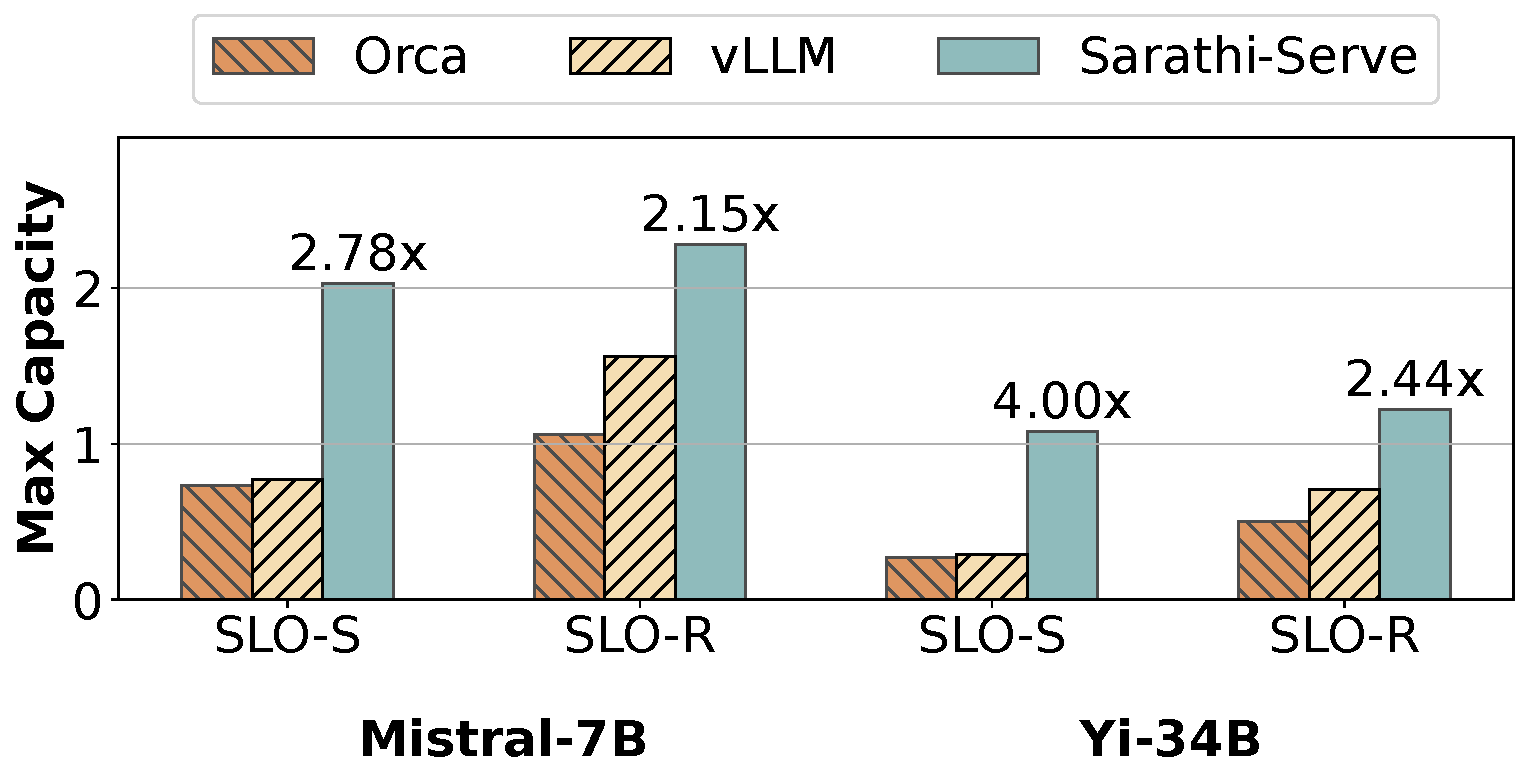
\includegraphics[width=0.95\textwidth]{figures/capacity-plots-tp-openchat.pdf}
        \caption{Dataset: \sharegpt.}
        \label{fig:eval:capacity:tp:openchat}
    \end{subfigure}
    \\
    \begin{subfigure}[b]{0.5\textwidth}
        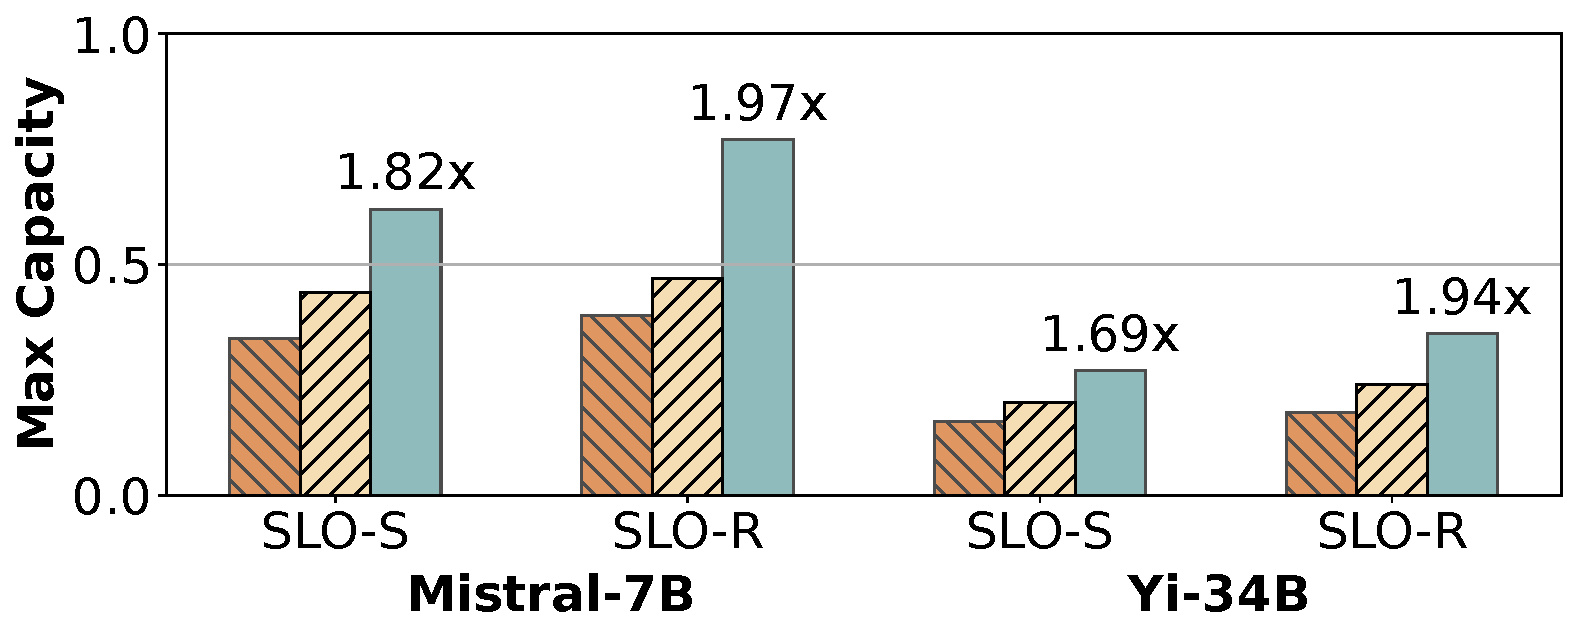
\includegraphics[width=0.95\textwidth]{figures/capacity-plots-tp-arxiv.pdf}
        \caption{Dataset: \arxivsum.}
        \label{fig:eval:capacity:tp:arxiv}
    \end{subfigure}
    \caption{Capacity (in queries per second) of \mistral and \yi with different schedulers under strict (SLO-S) and relaxed (SLO-R) latency SLOs.}
    \label{fig:eval:capacitytp}
\end{figure}


\subsection{Capacity Evaluation}
\label{sec-eval-capacity}
\begin{figure}[t]
    \begin{subfigure}[b]{0.5\textwidth}
        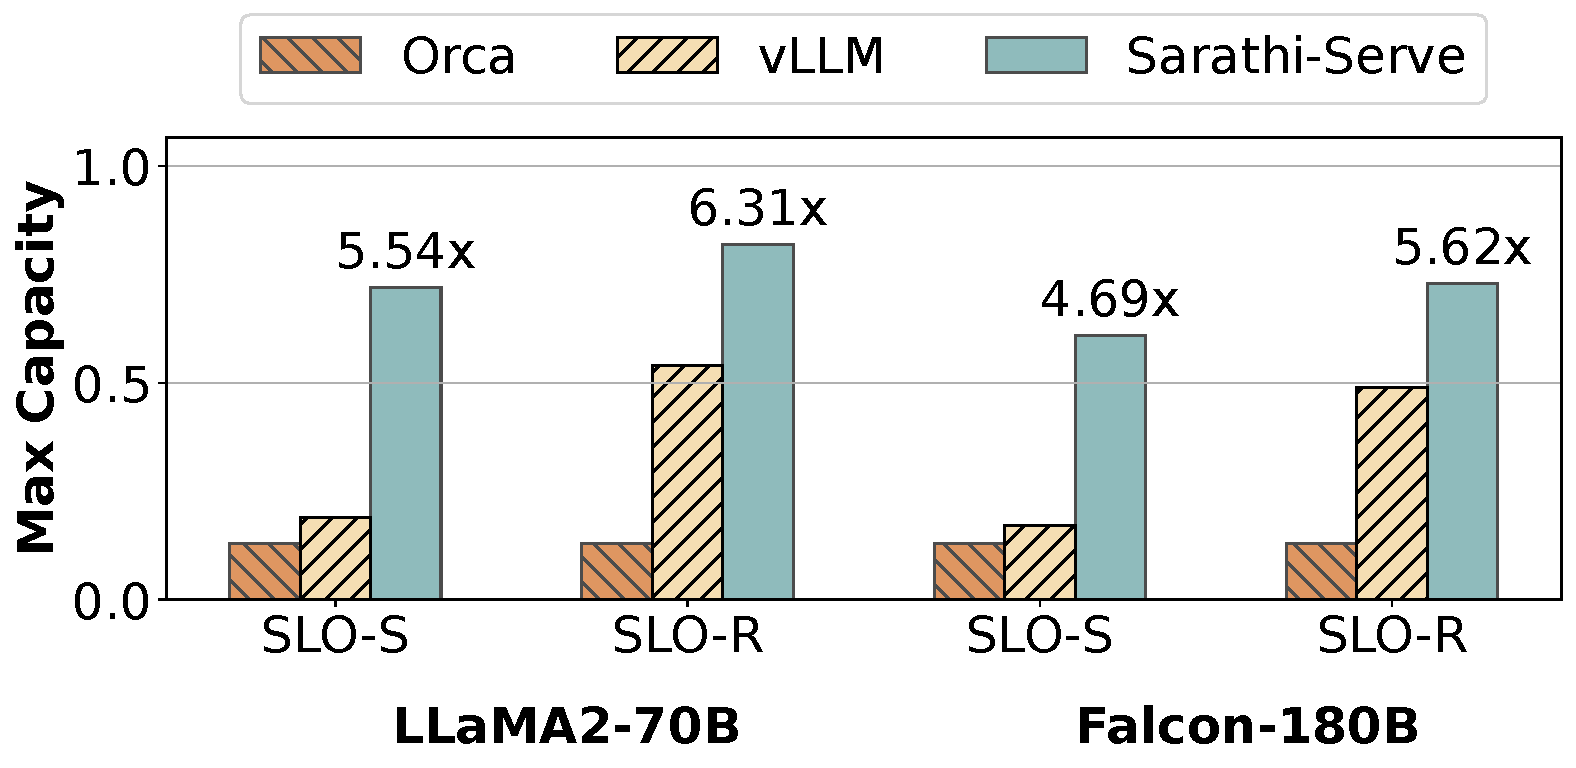
\includegraphics[width=0.95\textwidth]{figures/capacity-plots-pp-openchat.pdf}
        \caption{Dataset: \sharegpt.}
        \label{fig:eval:capacity:pp:openchat}
    \end{subfigure}
    \\
    \begin{subfigure}[b]{0.5\textwidth}
        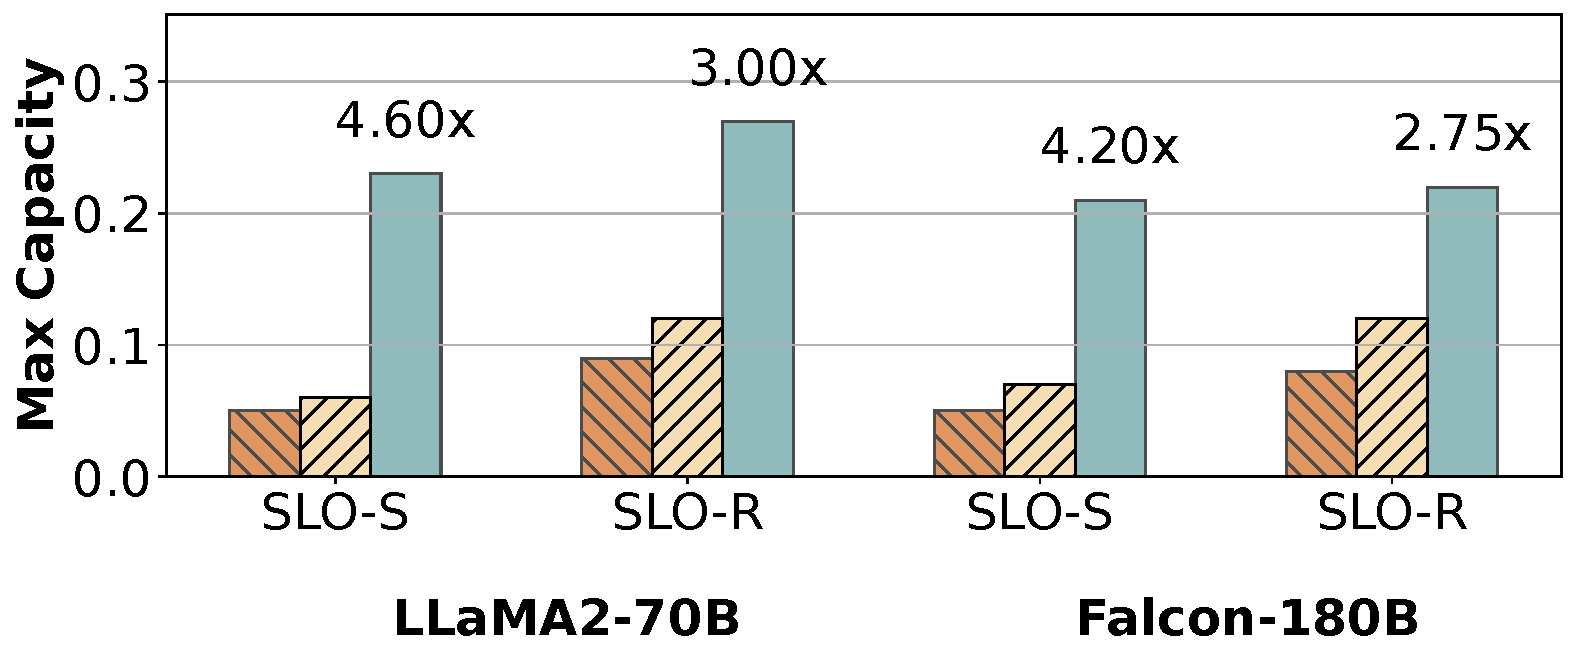
\includegraphics[width=0.95\textwidth]{figures/capacity-plots-pp-arxiv.pdf}
        \caption{Dataset: \arxivsum.}
        \label{fig:eval:capacity:pp:arxiv}
    \end{subfigure}
    \caption{Capacity of \llamaL and \falcon (models with pipeline parallelism) with different schedulers under strict (SLO-S) and relaxed (SLO-R) latency SLOs.}
    \label{fig:eval:capacitypp}
\end{figure}

We evaluate \sysname, Orca and vLLM on all four models and both datasets under two different latency configurations: \relaxed and \strict. Similar to Patel et al. \cite{patel2023splitwise}, to account for the intrinsic performance limitations of a model and hardware pair, we define the \slo on P99 TBT to be equal to 5\myx and 25\myx the execution time of a decode iteration for a request (with prefill length of 4k and 32 batch size) running without any prefill interference for the \strict and \relaxed settings, respectively. %
~\autoref{table:eval:slos} shows a summary of the absolute \slo thresholds. Note that the \strict SLO represents the latency target desired for interactive applications like chatbots. On the other hand, the \relaxed configuration is exemplary of systems where the complete sequence of output tokens should be generated within a predictable time limit but the TBT constraints on individual tokens is not very strict. For all load experiments, we ensure that the maximum load is sustainable, i.e., the queuing delay does not blow up (we use a limit of 2 seconds on median scheduling delay).


\autoref{fig:eval:capacitytp} and~\autoref{fig:eval:capacitypp} show the results of our capacity experiments. \sysname consistently outperforms Orca and vLLM in all cases across models and workloads. Under \strict \slo, \sysname can sustain up to $4.0\times$ higher load compared to Orca and $3.7\times$ higher load than vLLM under \strict \slo (\yi, \sharegpt). For larger models using pipeline parallelism, \sysname achieves gains of up to 6.3\myx and 4.3\myx compared to Orca and vLLM respectively (\llamaL, \sharegpt) due to few pipeline bubbles.


We observe that in most scenarios, Orca and vLLM violate the P99 TBT latency \slo before they can reach their maximum serviceable throughput. Thus, we observe relaxing the latency target leads to considerable increase in their model serving capacity. In \sysname, one can adjust the chunk size based on the desired SLO. Therefore, we use a strict token budget and split prompts into smaller chunks when operating under \strict latency \slo. This reduces system efficiency marginally but allows us to achieve lower tail latency. On the other hand, when the latency constraint is relaxed, we increase the token budget to allow more efficient prefills. We use token budget of 2048 and 512 for all models under the \relaxed and \strict settings,  respectively, except for the \llamaL \relaxed configuration where we use token budget of 1536 to reduce the impact of pipeline bubbles. The system performance can be further enhanced by dynamically varying the token budget based on workload characteristics. We leave this exploration for future work.


We further notice that vLLM significantly outperforms Orca under relaxed setting. The reason for this is two-fold. First, Orca batches prompts for multiple requests together ({\it max sequence length * batch size} compared to {\it max sequence length} in vLLM), which can lead to even higher tail latency in some cases. Second, vLLM supports a much larger batch size compared to Orca. The lower batch size in Orca is due to the lack of PagedAttention and the large activation memory footprint associated with processing batches with excessively large number of tokens.

Finally, note that the capacity of each system is higher for \sharegpt dataset compared to the \arxivsum dataset. This is expected because prompts in the \arxivsum datasets are much longer - 7059 vs 1730 median tokens as shown in~\autoref{table:eval:datasets}. The larger prompts makes Orca and vLLM more susceptible to latency violations due to higher processing time of these longer prefills.%



 \subsection{Throughput-Latency Tradeoff}
\label{subsec-tput-latency}

To fully understand the throughput-latency tradeoff in LLM serving systems, we vary the P99 TBT latency SLO and observe the impact on system capacity for vLLM and \sysname. ~\autoref{fig:eval:lateny-tput-tradeoff} shows the results for \mistral and \yi models with five different SLO values for the \sharegpt dataset.

We evaluate vLLM with three different batch sizes in an attempt to navigate the latency-throughput trade-off as prescribed by Yu et al. \cite{orca}. The maximum capacity of vLLM gets capped due to generation stalls under stringent TBT SLOs. Notably, the capacity of vLLM remains largely identical for all the three batch size settings. This implies that even though PagedAttention enables large batch sizes with efficient memory management -- in practical situations with latency constraints, vLLM cannot leverage the large batch size due to the steep latency-throughput tradeoff made by it's \prefillprio scheduler.

On the other hand, the latency-throughput tradeoff in \sysname can be precisely controlled by varying the token budget. \sysname achieves 3.5\myx higher capacity compared to vLLM under strict SLO (100ms, \mistral) using a small token budget of 512. For scenarios with more relaxed SLO constraints, picking a larger token budget of 2048 allows \sysname to operate more efficiently resulting in 1.65\myx higher capacity compared to vLLM (1s, \yi).







\begin{figure}[t!]
\centering
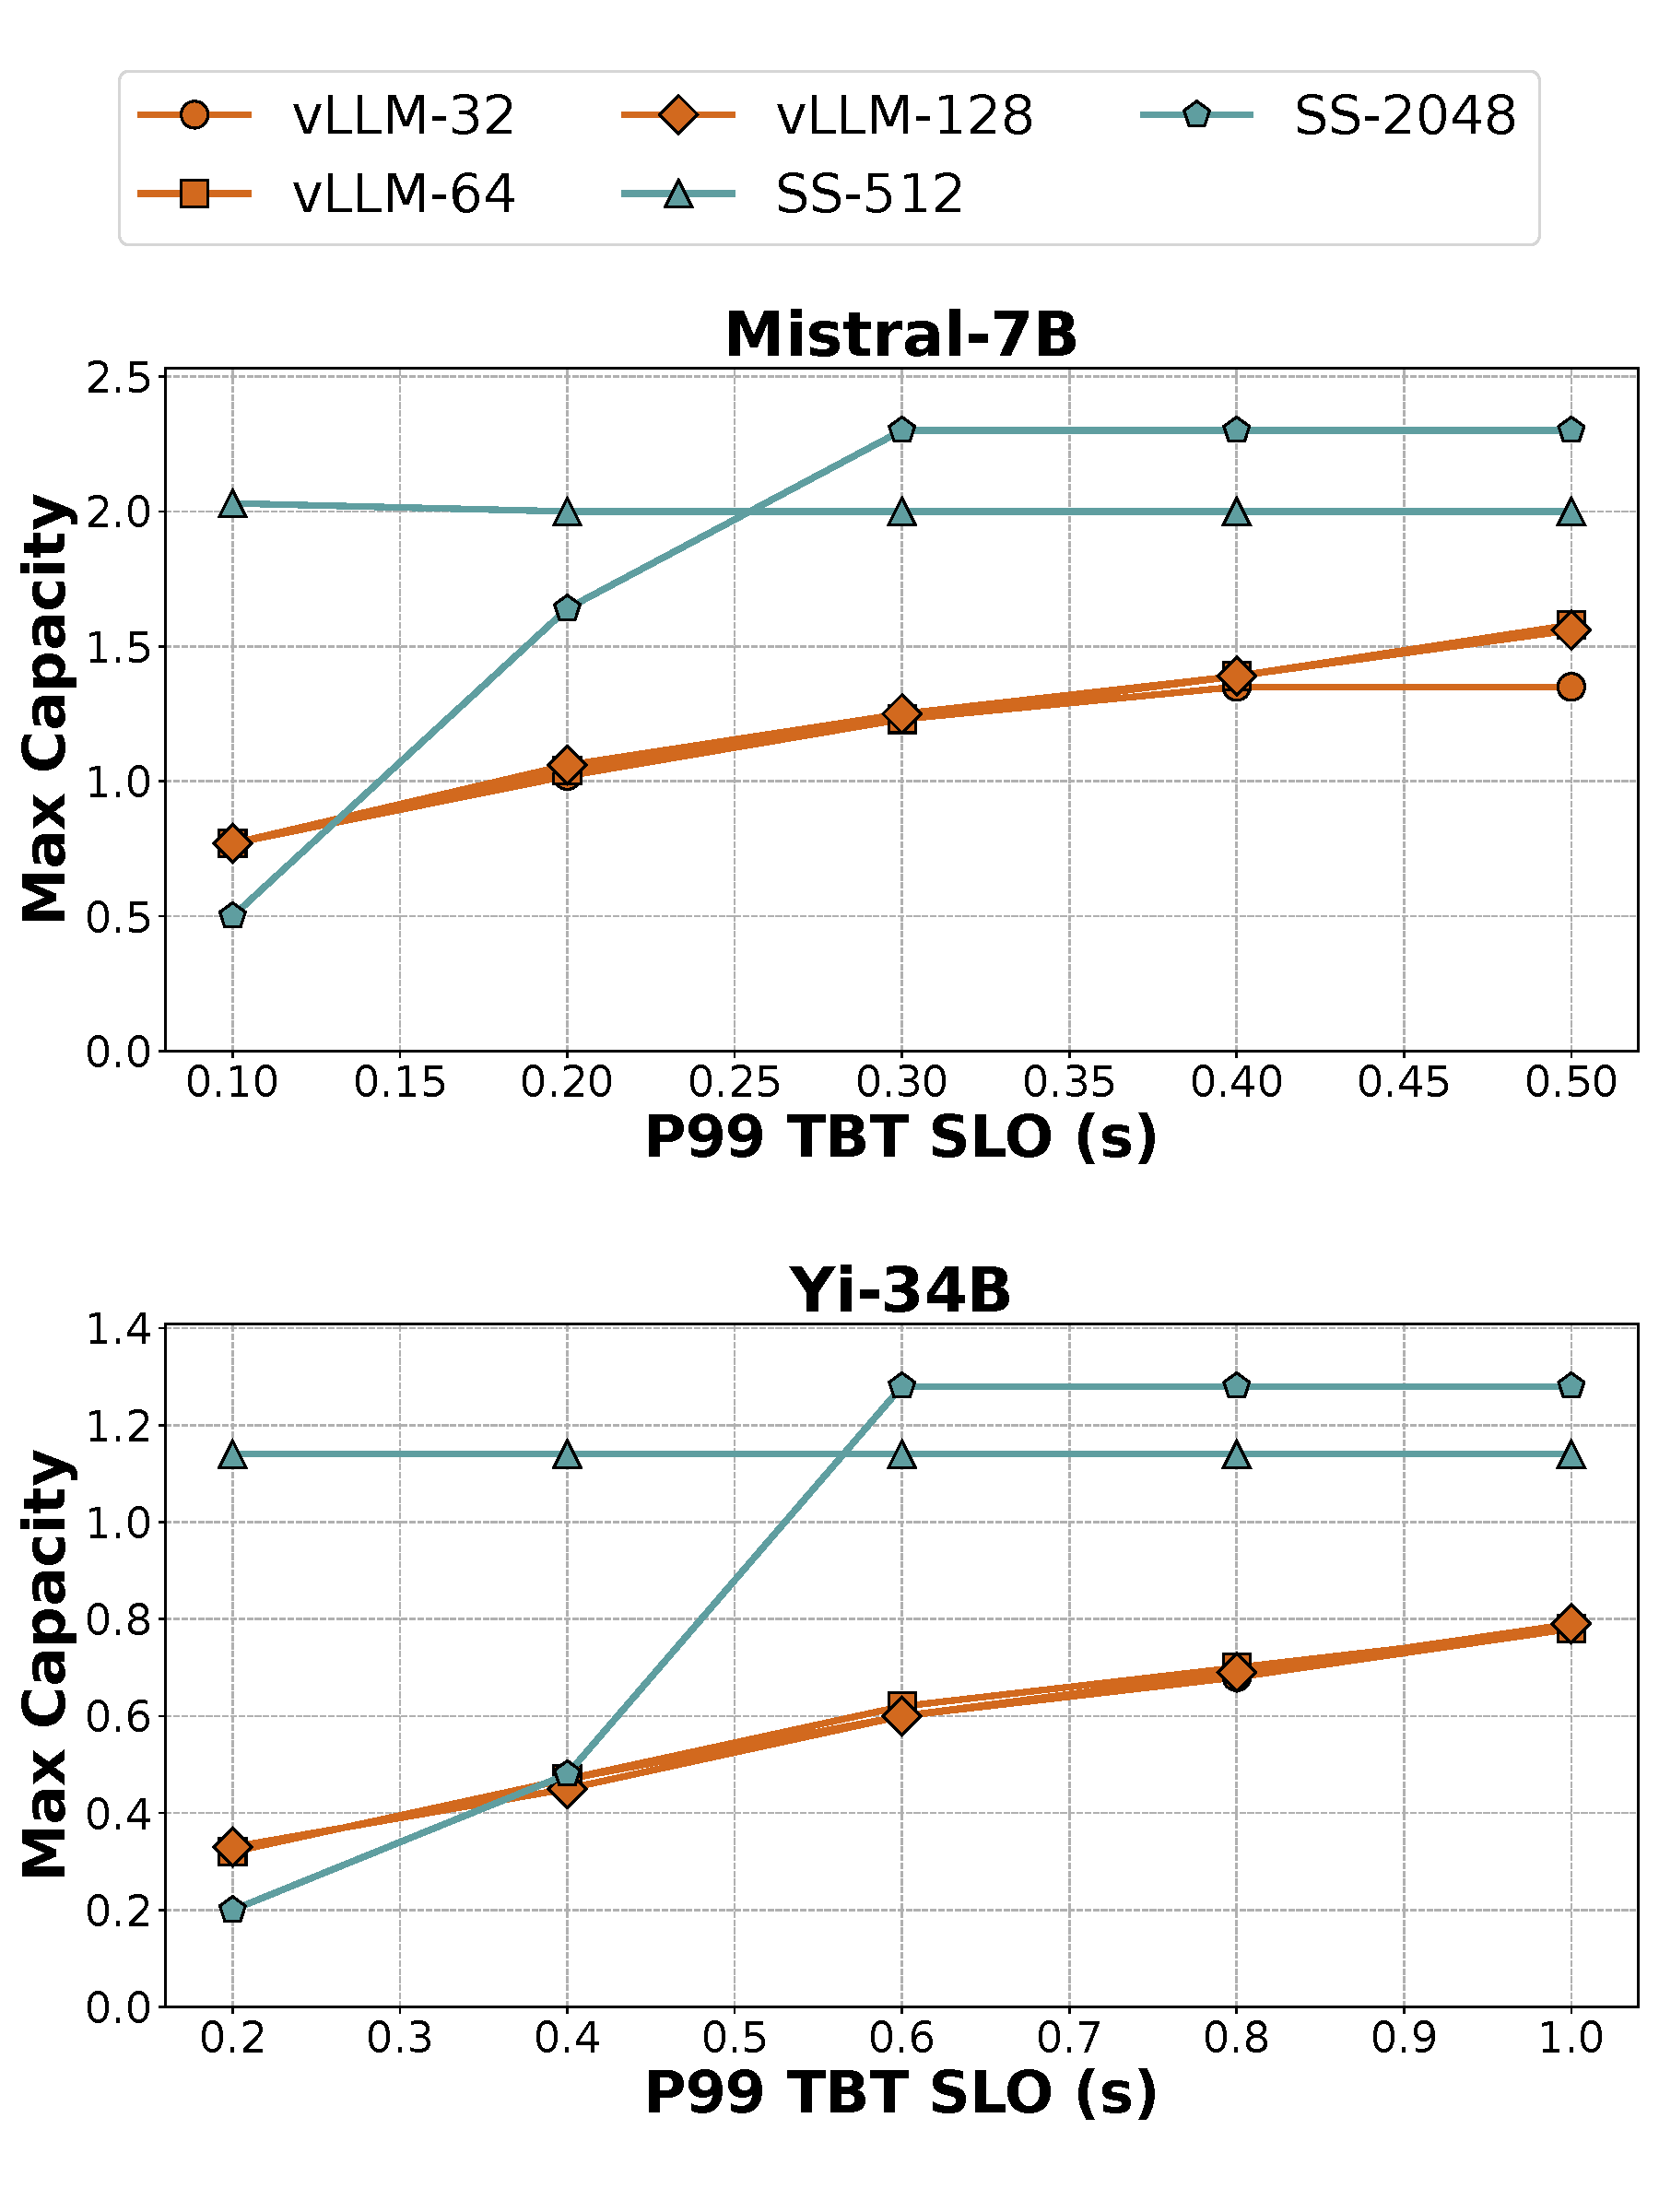
\includegraphics[width=0.95\linewidth]{figures/latency_tradeoff.pdf}
    \caption{Latency -- Throughput tradeoff in vLLM and \sysname for \mistral and \yi models on \sharegpt dataset. We evaluate vLLM with three different max batch sizes of 32, 64 and 128. For \sysname, we consider token budget of 512 and 2048 with max batch size of 128.
    \sysname delivers 3.5\myx higher capacity under stringent SLOs for \yi using \Hbatch.}
    \label{fig:eval:lateny-tput-tradeoff}
\end{figure}


\subsection{Making Pipeline Parallel Viable}
\label{sec-eval-pp}

We now show that \sysname makes it feasible to efficiently serve LLM inference across commodity networks with efficient pipeline parallelism. For these experiments, we run Falcon-180B over two nodes, each with four A100 GPUs, connected over 100 Gbps Ethernet. We evaluate model capacity under three configurations: vLLM with 8-way TP, vLLM with our pipeline-parallel implementation and \sysname with pipeline-parallel. For PP configurations, we do 4-way TP within node and 2-way PP across nodes.

\autoref{fig:eval:tp-latency} shows the latency for decode-only batches for Falcon-180B with purely tensor parallel TP-8 deployment compared to a TP-4 PP-2 hybrid parallel configuration. We observe that the median latency for tensor parallelism is $\sim 2$\myx higher than pipeline parallelism. This is because TP incurs high communication overhead due to cross-node all-reduces.


\autoref{fig:eval:pp-tp-capacity} shows the capacity for tensor and hybrid parallel configurations for Falcon-180B on \sharegpt dataset. Note that unlike the hybrid parallel configuration, TP achieves low capacity even under the \relaxed \slo due to high latency. Even though vLLM can support a fairly high load with hybrid parallelism under \relaxed \slo, it's performance drops sharply under the \strict regime due to pipeline bubbles. \sysname on the other hand, leverages \chunking to reduce the variation in the execution time between microbatches to avoid pipeline bubbles, resulting in a 1.48\myx increase in capacity under \relaxed \slos and 3.6\myx increase in capacity under \strict \slos.


\begin{figure}[t!]
\centering
\begin{subfigure}{0.235\textwidth}
    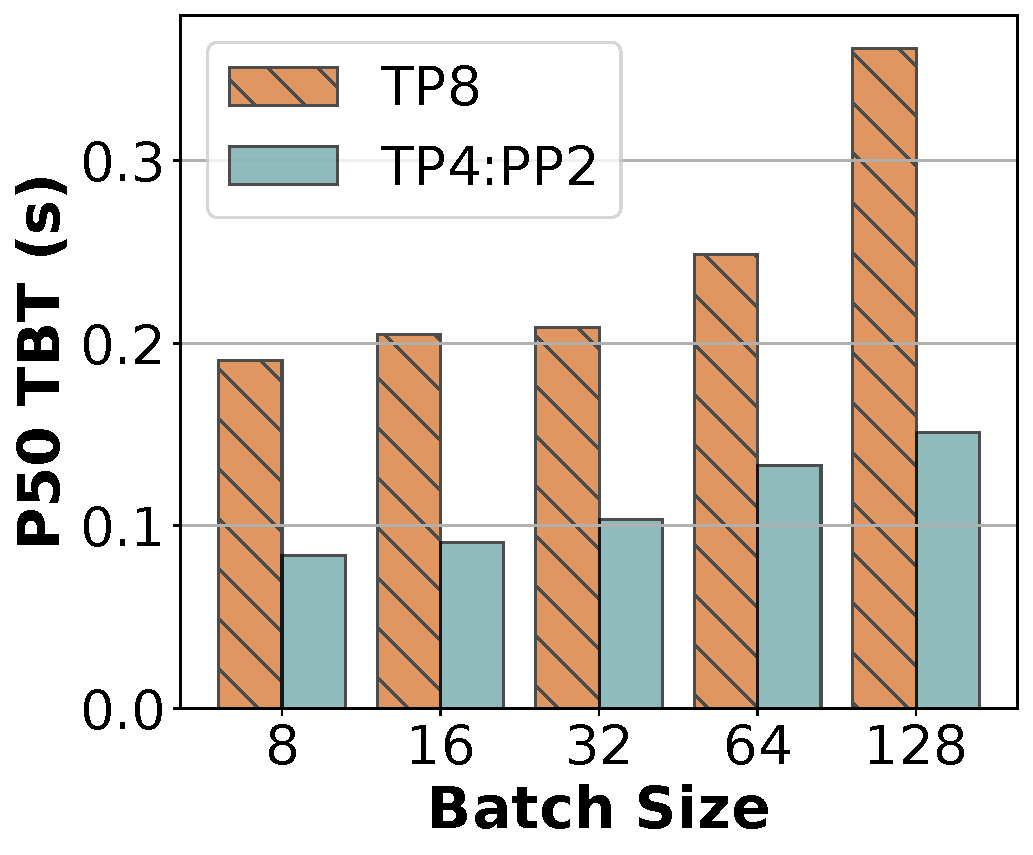
\includegraphics[width=\textwidth]{figures/pp-tp-latency.pdf}
    \caption{TBT (Falcon-180B).}
    \label{fig:eval:tp-latency}
\end{subfigure}
\begin{subfigure}{0.235\textwidth}
    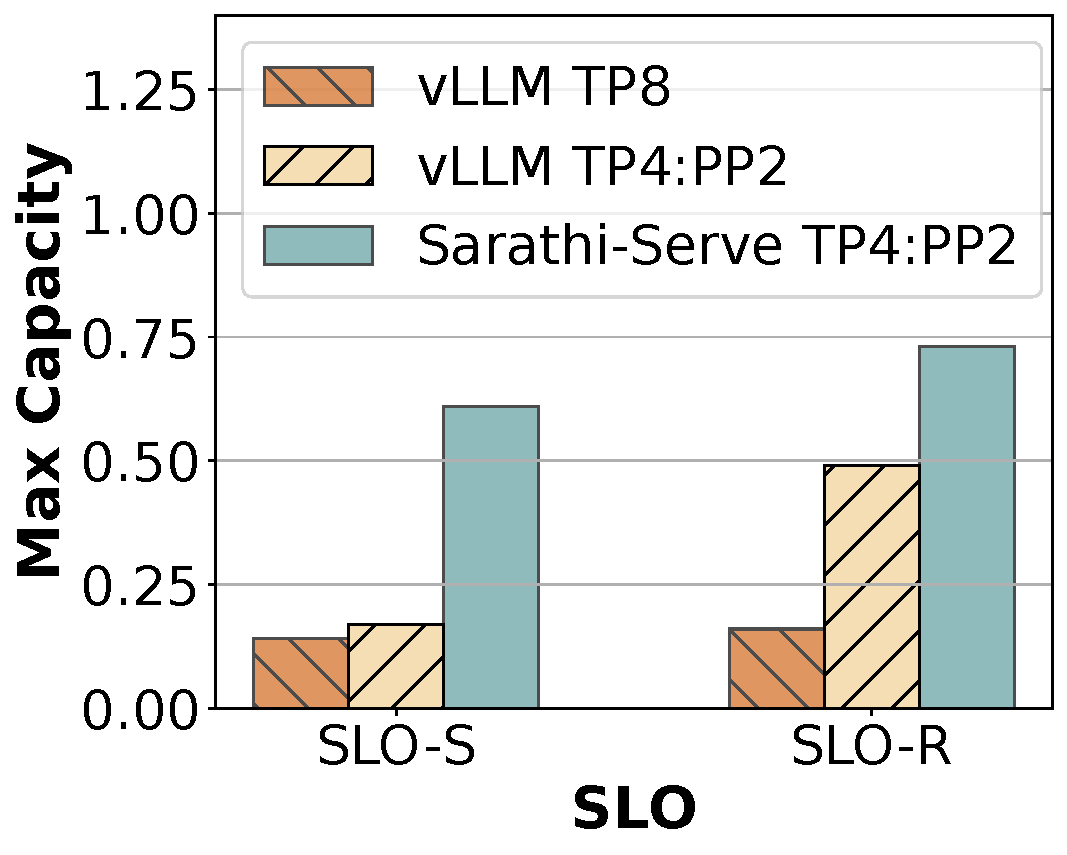
\includegraphics[width=\textwidth]{figures/pp-tp-capacity.pdf}
    \caption{Capacity (Falcon-180B).}
    \label{fig:eval:pp-tp-capacity}
\end{subfigure}
    \caption{TP scales poorly across nodes. (a) Median TBT for decode-only batches: cross node TP increases median TBT by more than $2\times$ compared to a 4-way TP within node and PP across nodes. (b) Capacity under strict (SLO-S) and
relaxed (SLO-R) latency SLOs: \sysname increases Falcon-180B's serving capacity by $4.3\times$ and $3.6\times$ over vLLM's TP-only and hybrid-parallel configurations under strict SLOs.}
    \label{fig:enter-label}
\end{figure}

\subsection{Ablation Study}
\label{sec-eval-ablation}


In this subsection, we conduct an ablation study on different aspects on \sysname. In particular, we are interested in answering the following two questions: 1) what is the effect of chunking on prefill throughput, and 2) analyzing the impact of hybrid-batching and chunking on latency. While we provide results only for a few experiments in this section, all the trends discussed below are consistent across various model-hardware combinations.

\subsubsection{Overhead of \chunking}
\label{sec-eval-ablation1}

\autoref{fig:eval:ablation:overheads} shows how much overhead chunking adds in \yi{} -- on overall prefill runtime. As expected, smaller chunks introduce higher overhead as shown by the gradually decreasing bar heights in~\autoref{fig:eval:ablation:overheads}. However, even with the smallest chunk size of 512, we observe a moderate overhead of at most $\sim$25\%. Whereas with the larger token budget of 2048, chunked prefills have almost negligible overhead. %









\begin{figure}[t!]
    \centering        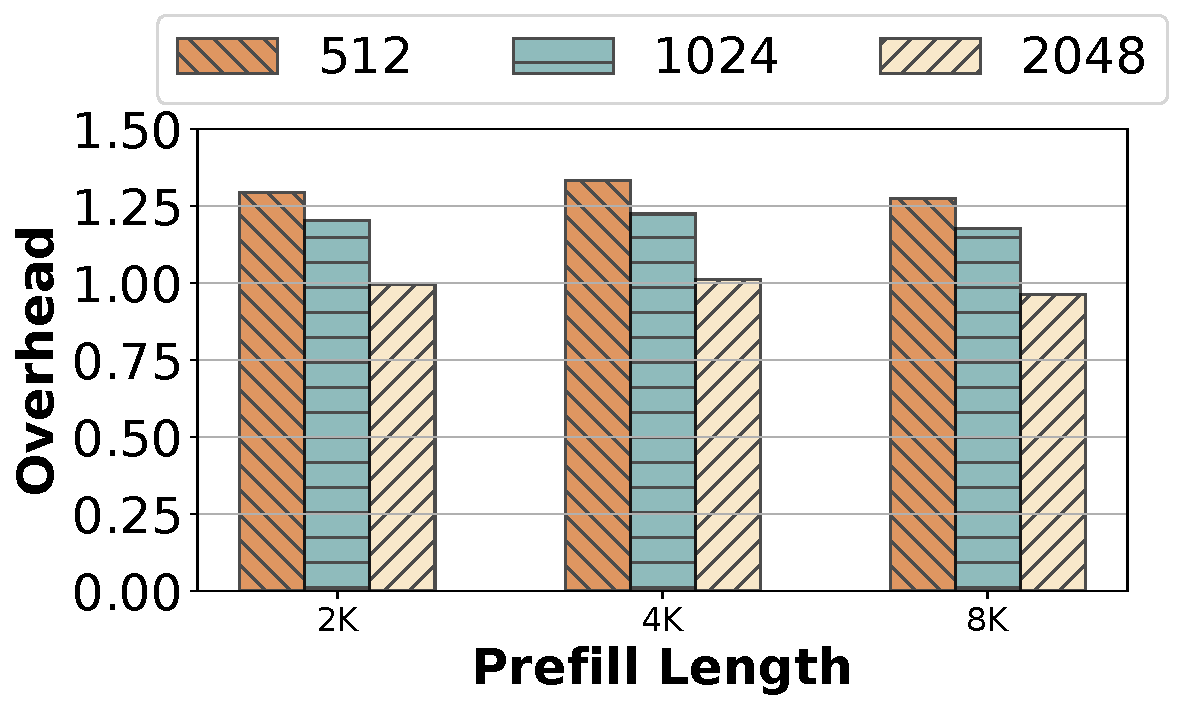
\includegraphics[width=0.38\textwidth]{figures/chunking-overhead.pdf}
    \caption{Overhead of \chunking in prefill computation for Yi-34B (TP-2) normalized to the cost of no-chunking, shown for various prompt lengths using chunk lengths of 512, 1024 and 2048.}
    \label{fig:eval:ablation:overheads}
\end{figure}



\begin{table}[t]
\centering
\setlength{\tabcolsep}{2pt}
\scalebox{0.85}{
\begin{tabular}{c|cc|cc}
\textbf{Scheduler} & \multicolumn{2}{c|}{\textbf{\sharegpt}} & \multicolumn{2}{c}{\textbf{\arxivsum}} \\
\cline{2-3} \cline{4-5}
& P50 TTFT & P99 TBT & P50 TTFT & P99 TBT \\ \toprule
\dcoel{}\textit{-only} & 0.53 & 0.68 & 3.78 & 1.38 \\
\chunking{}\textit{-only} & 1.04 & 0.17 & 5.38 & 0.20 \\
\sysname (combined) & 0.76 & 0.14 & 3.90 & 0.17 \\
\bottomrule
\end{tabular}}
\caption{TTFT and TBT latency measured in seconds for \dcoel and \chunking used in isolation as well as when they are used in tandem, evaluated over 128 requests for Yi-34B running on two A100s with a token budget of 1024. By using both \dcoel and \chunking, \sysname is able to lower both TTFT and TBT.}
\label{table:eval:attribution}
\end{table}


\subsubsection{Impact of individual techniques}
\label{sec-eval-ablation2}
Finally, \autoref{table:eval:attribution} shows the TTFT and TBT latency with each component of  \sysname evaluated in isolation \ie \chunking-only, \dcoel-only (mixed batches with both prefill and decode requests) and when they are used in tandem. These results show that the two techniques work best together: \chunking-only increases TTFT as prefill chunks are slightly inefficient whereas \dcoel-only increases TBT because long prefills can still create generation stalls. When used together, \sysname improves performance along both dimensions.



